After the first MapReduce phase is completed, the skyline candidate object set $O_c$ is collected. In the next step, the final skyline probability of every object is necessary to compute for determining $p-$skyline objects,  Before we illustrate our merging algorithm for filtering $O_c$, we firstly study the data distribution of remained candidate objects after the first MapReduce phase.

\subsection{Shape Analysis}

\begin{figure*}[!t]
    \begin{center}
    \vspace{-1.5pc}
  \subfigbottomskip = 2pt \subfigure[Independent Distribution]
    {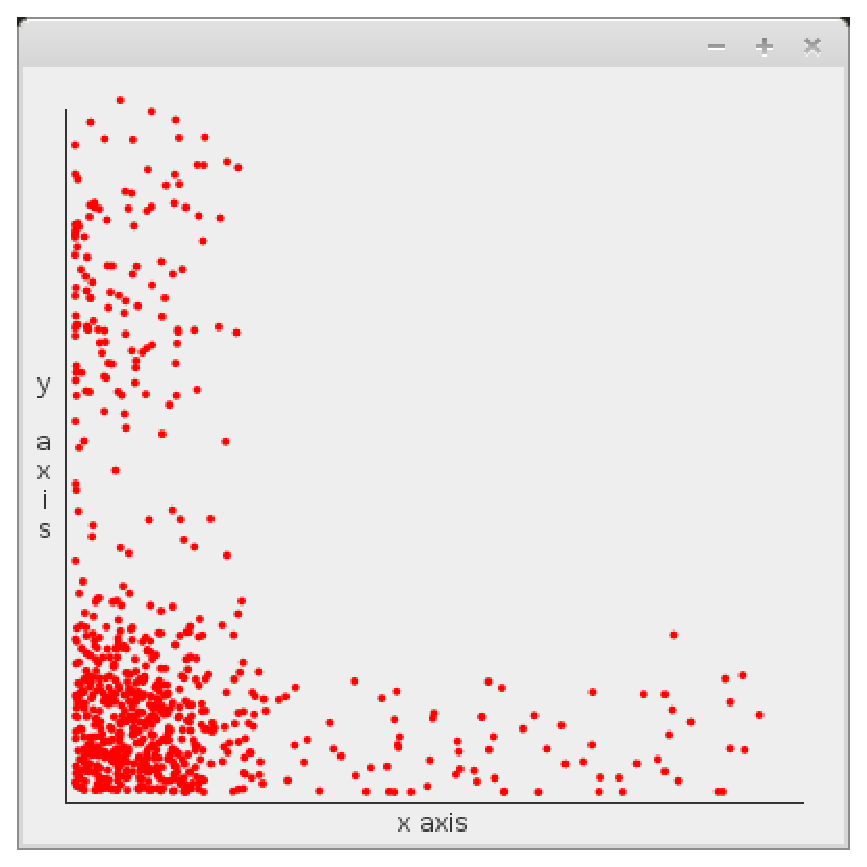
\includegraphics[width=0.24\textwidth]{figs/inde.eps}}
    \hspace{0.01em}
  \subfigbottomskip = 2pt  \subfigure[Anti-correlated Distribution]
    {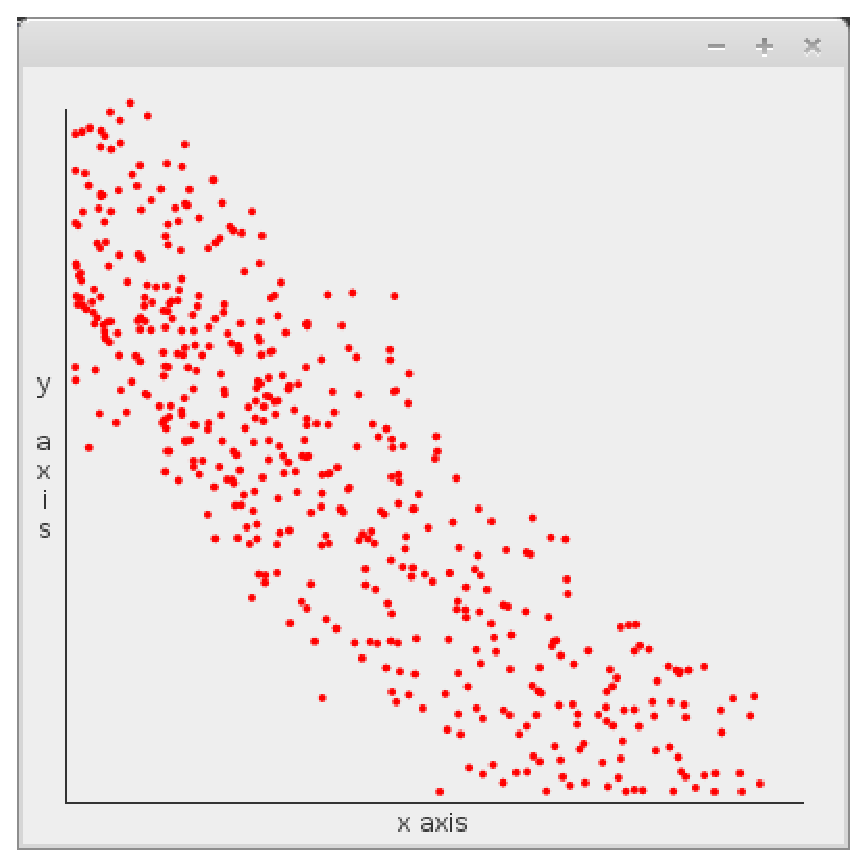
\includegraphics[width=0.24\textwidth]{figs/anti.eps}}
    \hspace{0.01em}
  \subfigbottomskip = 2pt  \subfigure[Correlated Distribution]
    {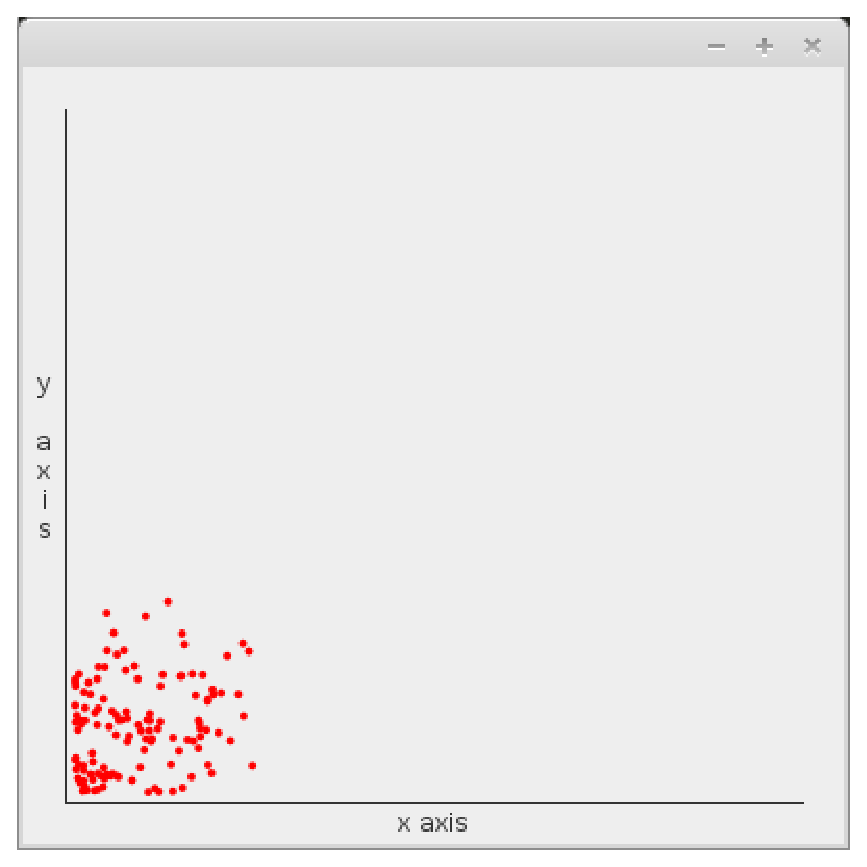
\includegraphics[width=0.24\textwidth]{figs/corr.eps}}

    \caption{Data Point Distribution after phase 1.}
    \label{fig:shape}
    \end{center}
\vspace{-10pt}
\end{figure*}

Since the angle-based pruning only knows the local data at a fixed region, the objects remained in a region decide the final step of merging. Therefore, we study the shape of instance distribution after the first MapReduce phase. To evaluate this, we conducted an experiment to depict the shape of instance distribution. Figure~\ref{fig:shape} shows the three figures, each of which depicts an instance distribution. The detailed experiment parameters are illustrated as follows. In the two-dimensional space, objects are distributed between [0, 1] in each domain. Three types of object distribution are independent distribution, correlated distribution, and anti-correlated distribution respectively. The cardinality of objects is 5000. For each object, instances are created under a rectangle region, the edge size of which follows a normal distribution in range [0, 0.2] with expectation 0.1 and standard deviation 0.025
The number of instances in each object follows uniform distribution in range [1, 100]. we evenly split the first quadrant into 6 angles, and skyline probability is computed in each angle region using the algorithm in the first MapReduce. After that, we collected the objects which are still remained in each region, and put all of them in the x-y axis.

In Figure~\ref{fig:shape}, three types of object distribution exhibit different data distributions. In Independent or Anti-correlated distribution of data, there are still many instances remained. Therefore, the Strategy proposed in the merging phase should be able to apply in every case if data distribution, especially for Independent and Anti-correlated Distribution data.

\subsection{Rectangle Splitting}
\begin{figure}[t]
\vspace{-15pt}
\centering
  \centerline{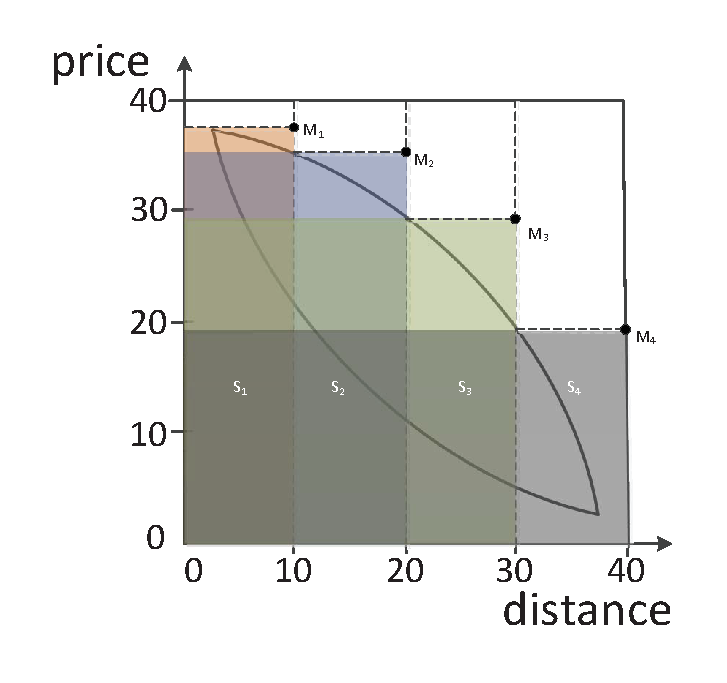
\psfig{file=figs/grid-merge.eps,width=4.0in}}
  \caption{Merging Phase}
  \vspace{-15pt}
  \label{figure:gridMerge}
\end{figure}

In this section, we devise an approach to efficiently evaluate skyline probability for those remained objects. To utilize the MapReduce framework, we partition remained data to several domains which are able to work individually. The general idea is to split data into several partitions, and each partition is not affected by others. Take Figure~\ref{figure:gridMerge} as an example. Assume the remained instances form the anti-correlated distribution. X axis is evenly split into 4 partitions $S_1, S_2, \dots, S_4$, and 4 maximum coordinate points are computed for each partition. Each point is dominated by any instance in this partition. Then each grid region is rounded by the origin and the maximum point. In Figure~\ref{figure:gridMerge}, green area represents only instances which dominate the instances in $S_3$. Therefore, for computing instance skyline probability in $S_3$, it only needs instances in green area.

Followed by the example introduced above, the data is partitioned based on evenly along the x-axis. Given the the number of reducers $n$, the data is partitioned into n parts. Meanwhile, mapping method groups data into $N$ groups. Every group has two types of data, instances in $C_o$ and $I$ respectively. Take Figure~\ref{figure:gridMerge} as an example. The instances of $C_o$ in $S_2$ is in $S_2$ rectangle, and instances in the blue area are instance set $I$, which dominates $C_o$. Based on the grouping scheme, the mapping phase maps the two types of data to every slave machine. It is obvious that the choice of $n$ affects the efficiency of skyline probability computing. In the experiment section, we observe the performance trend with the variety of $n$.

In the reduce phase, skyline probability of every instance is computed. Assume an instance $p$ is in a partition $V^A$. Since $p$ is only dominated by corresponding region of instances, the instance skyline probability $SkyProb(p)$ is obtained using the standard approach. It finds all instances which instance $p$ by iterating all instances in this partition, and do Equations introduced in the Section~\ref{sec:prelim}. Then instance skyline probability of every instance is exported to a file in each partition.

After every instance in $C_o$ obtains its instance skyline probability, the second phase is completed. object skyline probability is grouped by iterating all instance skyline probability by Equation~\ref{equ_final}. $p-$skyline objects area able to be obtained by retrieving objects whose object skyline probability is larger than or equal to $p$.

